\documentclass[12pt]{report}

\usepackage[english]{babel}
\usepackage[utf8x]{inputenc}
\usepackage{amsmath}
\usepackage{graphicx}
\usepackage{multirow}
\usepackage[hypcap]{caption}
\usepackage{setspace} 
\usepackage{float}

\title{Lab 7: Ceramics and Glasses}
\author{Zachary Tschirhart \\
	\small \\
        \small EID: zst75 \\
	\small Department of Aerospace Engineering and Engineering Mechanics \\
	\small \textbf{ASE 324L (Mon 2:00-5:00)} \\
	\small Unique: 13740}
\date{March 24, 2014}


\begin{document}
\maketitle

\setcounter{secnumdepth}{0}

\section{Results and Discussion}
\doublespacing

\subsection{Question 1}

Using the equation from 8.1 and the rectangle equation from figure 8.6, the following equations can be realized for stress and strain.

\begin{equation}
  \sigma = \frac{3FL}{2bd^2}
  \label{equation:equation1}
\end{equation}

\begin{equation}
  \epsilon = \frac{6d\delta}{L^2}
  \label{equation:equation1}
\end{equation}

Where b is the width of the specimen, d is the thickness, and L is the length. 

\subsection{Question 2}

The plot was created from all specimen collected from the labs using the equations from question 1. 
\begin{figure}[H]
	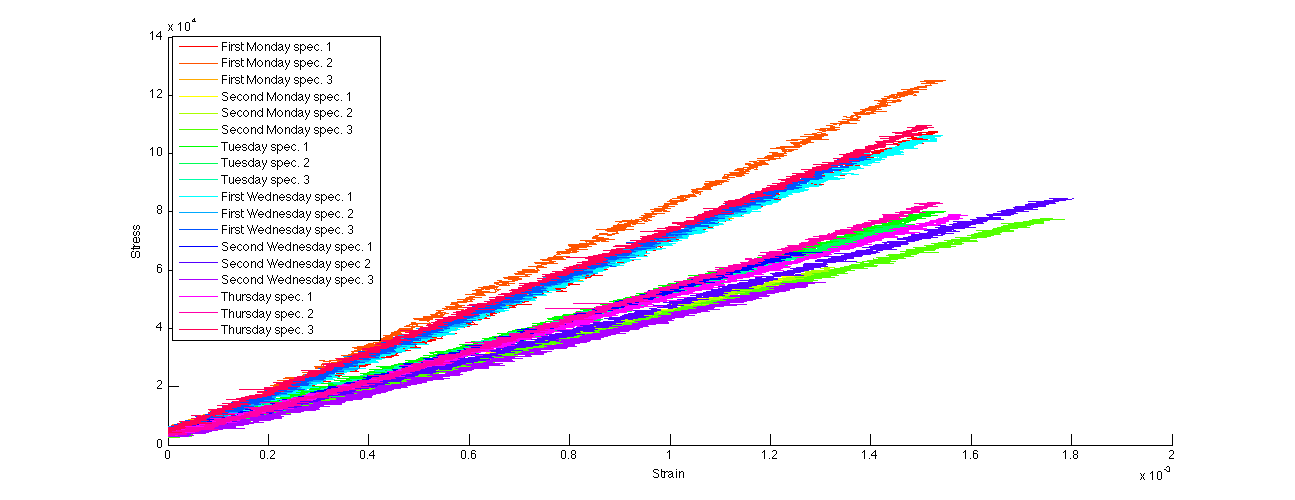
\includegraphics[width=1\textwidth]{problem2.png}
	\caption{Stress vs. strain diagrams from the eighteen specimen.}
	\label{fig:Figure1}
\end{figure}

In order to get the mean elastic modulus and flexural strength, a least squares fit was used for each specimen data set. Then the slope and end points were averaged.

The average elastic modulus was 56.12e6 psi and the average flexural strength was 83.32 ksi

These results are close to the manufacture specs of 56.56e6 psi for elastic modulus and not so close to the 43.51 ksi for the flexural strength. 

\subsection{Question 3}
Since the theoretical force required to break that specimen is 7853.98 N, then the chances that this force would not be enough to fracture the specimen. There is still a chance that the specimen would fracture, since the micro-fractures could be aligned in such a way that could cause a significant weakness. 

\subsection{Question 4}
Using equations 8.2, 8.3 and the mass density for porous material, the plots below can be made.

\begin{figure}[H]
	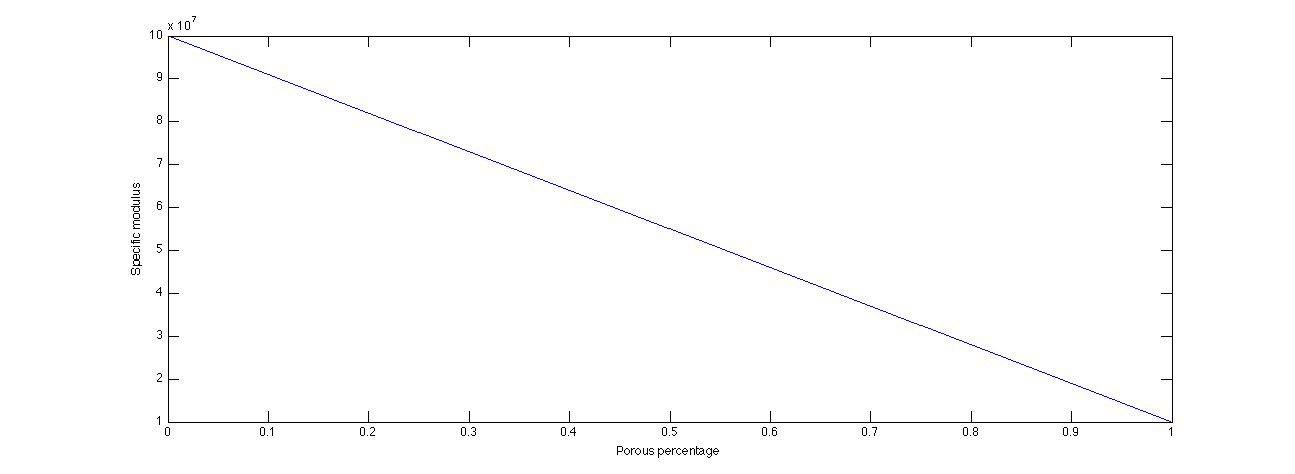
\includegraphics[width=1\textwidth]{problem4a.png}
	\caption{Specific modulus vs. porosities}
	\label{fig:Figure2}
\end{figure}

\begin{figure}[H]
	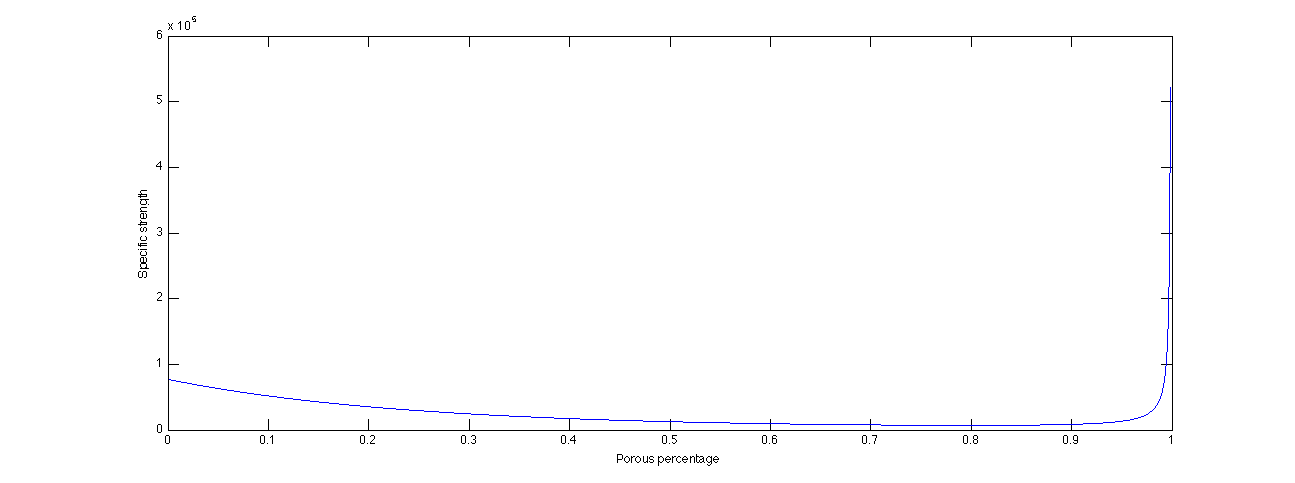
\includegraphics[width=1\textwidth]{problem4b.png}
	\caption{Specific strength vs. porosities}
	\label{fig:Figure3}
\end{figure}

The porous percentage at which specific modulus maximizes is at zero percentage, and around 100 percent for specific strength. The maximum specific strength is around one hundred percent because the function blows up around one hundred percent, otherwise it is maximized near zero percent 

\subsection{Question 5}

The Weibull distribution for ceramic strength plot is below:
\begin{figure}[H]
	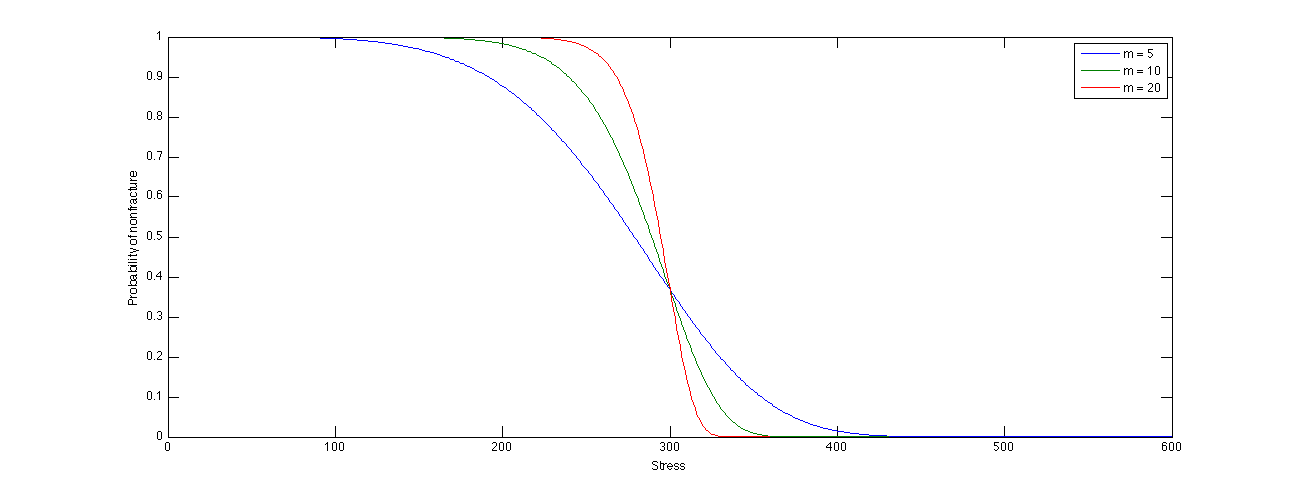
\includegraphics[width=1\textwidth]{problem5.png}
	\caption{Weibull distributions for moduli 5, 10, and 20}
	\label{fig:Figure4}
\end{figure}

The possible statistical scattering of the strength data for different Weibull moduli could be coming from the fact that not all specimen will break as this function dictates. This Function only tries to fit to the fracture at specific stresses, but it is not exact. This is where the scattered points come from.

\end{document}
